\section{Electrical Characterisation of Silicon Sensors}
\label{sec:setup}

\subsection{Setup}
\label{subsec:setup_principle}

\begin{figure}[h]
	\centering
	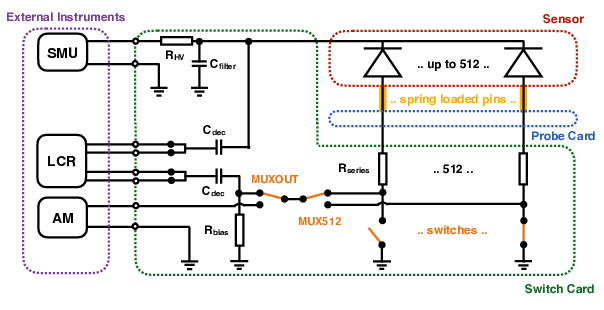
\includegraphics[width=0.75\textwidth]{figures/circuit_cards_updated.png}
	\caption{
		Circuitry of our tests, taken from~\cite{pitters:array2019}
	}
	\label{fig:switchprobecard_CAD}
\end{figure}


\begin{itemize}
	\item ARRAY system~\cite{pitters:array2019}
	\item Total leakage current over \SI{12}{\kilo\ohm} resistor leading to drop of effective bias voltage, which is corrected for
	\item Low frequency preferable to minimise influence on sensor, but associated to error minimal for 2kHz (SPICE simulation ARRAY paper), less than 10percent impact on depletion voltage, less than 2percent impact on final capacitance (cf. Philipp)
\end{itemize}

\begin{itemize}
	\item Cold station Wentworth + model
	\item Measurements conducted at low temperatures to prevent hight currents and to protect the system
\end{itemize}




\subsection{Measurement Procedure}
\label{subsec:setup_procedure}
\begin{itemize}
	\item 1st round: Per-pad leakage currents (IV), 2nd round: per-pad capacitance
	\item Unless stated otherwise: measurements at set chuck temperature of \SI{-40}{\celsius}
	\item Current compliances to protect system:
	\item Total current compliance: \SI{2}{\milli\ampere}
	\item Per-pad current compliance: \SI{5}{\micro\ampere}
	\item Cells in compliance masked in following leakage current measurements at higher voltages and skipped in subsequent capacitance measurement
	\item LCR frequency for capacitance measurement is \SI{2}{\kilo\hertz}
	\item Open-correction, serial definition of capacitance
	\item Iterate over all channels at constant voltage, then switch voltage
	\item Total characterisation time: IV = \SI{90}{\minute} (LD)
	\item Total characterisation time: CV = \SI{150}{\minute} (LD)

\end{itemize}